\tableofcontents
\section*{Предисловие}
При выполнении данной лабораторной работы было решено использовать 
\href{https://python-control.readthedocs.io/en/0.9.4/}{Python Control Systems Library}.
Данный инструмент является альтернативой Matlab, адаптированной для использования на 
языке Python и предоставляет широкий функционал для анализа и моделирования систем,
а также синтеза регуляторов для управления.

Полный листинг моделирования систем представлен в \href{https://github.com/diuzhevVlad/control-theory-itmo-fall-2023/blob/main/Lab12/Lab12.ipynb}{jupyter notebook} на GitHub.

\pagebreak

\section{Компенсирующий регулятор по состоянию}

Рассмотрим систему вида:
\begin{equation}
    \begin{cases}
        \dot{x} = A_1x + B_1u + B_2w \\
        z = C_2x
    \end{cases},
\end{equation}
где $w$:
\begin{equation}
    \dot{w} = A_2w
\end{equation}

Для данной системы можем синтезировать регулятор вида $u = K_1x + K_2w$, гарантирующий:
\begin{equation*}
    \lim_{t\to\infty} z(t) = 0
\end{equation*}

$K_1$ можем выбрать как матрицу регулятора, синтезированного любым способом. Матрицу $K_2$ найдем следующим образом:
\begin{equation}
    \begin{cases}
        PA_2 - A_1P = B_1Y + B_2\\
        C_2P + D_2 = 0 \\
        K_2 = Y - K_1P
    \end{cases}
\end{equation}

\begin{equation*}
    A_1 = \begin{bmatrix}
        0 & 1 & 0 & 0 \\
        0 & 0 & 1 & 0 \\
        0 & 0 & 0 & 1 \\
        0 & 0 & 2 & 0
    \end{bmatrix}, 
    B_1 = \begin{bmatrix}
        0 \\ 1 \\ 0 \\ 1
    \end{bmatrix},
    B_2 = \begin{bmatrix}
        0 & 0 & 0 & 0 \\
        1 & 0 & 1 & 0 \\
        0 & 0 & 0 & 0 \\
        2 & 0 & 2 & 0
    \end{bmatrix}, 
    A_2 = \begin{bmatrix}
        0 & 2 & 0 & 0 \\
        -2 & 0 & 0 & 0 \\
        0 & 0 & 0 & 3 \\
        0 & 0 & -3 & 0
    \end{bmatrix}, 
\end{equation*}
\begin{equation*}
    C_2 = \begin{bmatrix}
        0 & 0 & 1 & 0
    \end{bmatrix}.
\end{equation*}

Полученные матрицы регулятора ($K_1$ -- LQR):
\begin{equation*}
    K_1 = \begin{bmatrix}
        1 & 3.96 & -9.34 & -8.28
    \end{bmatrix},
    K_2 = \begin{bmatrix}
        -2.25 & -1.98 & -2.21 & -1.32
    \end{bmatrix}
\end{equation*}

Проведем моделирование системы:

\begin{figure}[h]
    \centering
    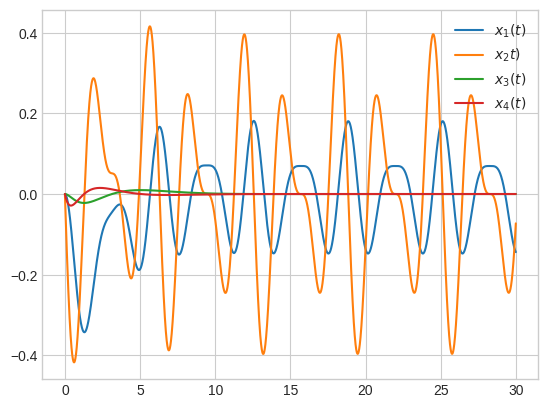
\includegraphics[width=300px]{task_1_states.png}
    \caption{\label{fig:task4_3_2}Задание 1. Вектор состояния.}
\end{figure}

\begin{figure}[]
    \centering
    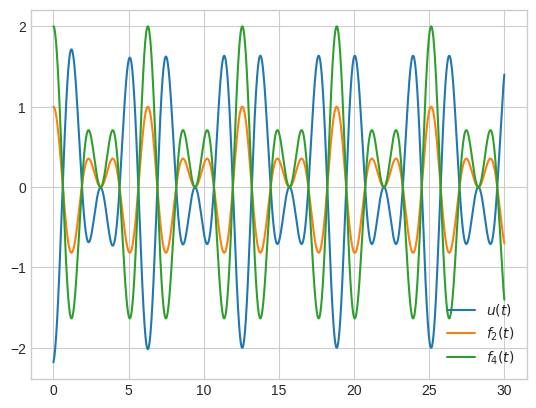
\includegraphics[width=300px]{task_1_compensation.png}
    \caption{\label{fig:task4_3_2}Задание 1. Управляющее воздействие и внешние возмущения.}
\end{figure}

\begin{figure}[]
    \centering
    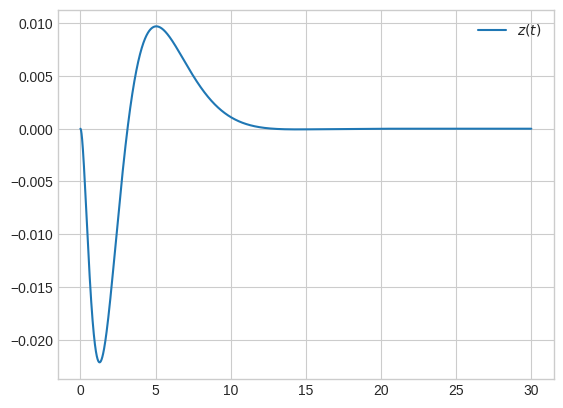
\includegraphics[width=300px]{task_1_outputs.png}
    \caption{\label{fig:task4_3_2}Задание 1. Регулируемый выход.}
\end{figure}

\pagebreak

\section{Следящий регулятор по состоянию}

Рассмотрим систему:
\begin{equation}
    \begin{cases}
        \dot{x} = A_1x + B_1u \\
        z = C_2x + D_2w
    \end{cases}
\end{equation}

\begin{equation*}
    A_1 = \begin{bmatrix}
        0 & 1 & 0 & 0 \\
        0 & 0 & 1 & 0 \\
        0 & 0 & 0 & 1 \\
        0 & 0 & 2 & 0
    \end{bmatrix}, 
    B_1 = \begin{bmatrix}
        0 \\ 1 \\ 0 \\ 1
    \end{bmatrix},
    A_2 = \begin{bmatrix}
        0 & 2 & 0 & 0 \\
        -2 & 0 & 0 & 0 \\
        0 & 0 & 0 & 1 \\
        0 & 0 & -1 & 0
    \end{bmatrix}, 
\end{equation*}
\begin{equation*}
    C_2 = \begin{bmatrix}
        0 & 0 & 1 & 0
    \end{bmatrix},
    D_2 = \begin{bmatrix}
        -1 & 0 & -2 & 0
    \end{bmatrix}.
\end{equation*}

Полученные матрицы регулятора ($K_1$ -- LQR):
\begin{equation*}
    K_1 = \begin{bmatrix}
        1 & 3.96 & -9.34 & -8.28
    \end{bmatrix},
    K_2 = \begin{bmatrix}
        2.09 & 6.66 & 8.68 & 0.72
    \end{bmatrix}
\end{equation*}

Проведем моделирование системы:

\begin{figure}[h]
    \centering
    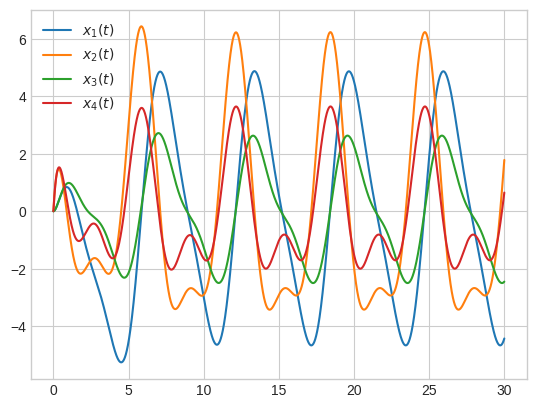
\includegraphics[width=300px]{task_2_states.png}
    \caption{\label{fig:task4_3_2}Задание 2. Вектор состояния.}
\end{figure}

\begin{figure}[]
    \centering
    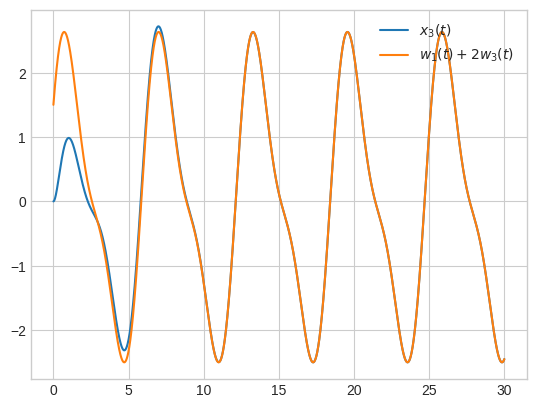
\includegraphics[width=300px]{task_2_tracking.png}
    \caption{\label{fig:task4_3_2}Задание 2. Слежение.}
\end{figure}

\begin{figure}[]
    \centering
    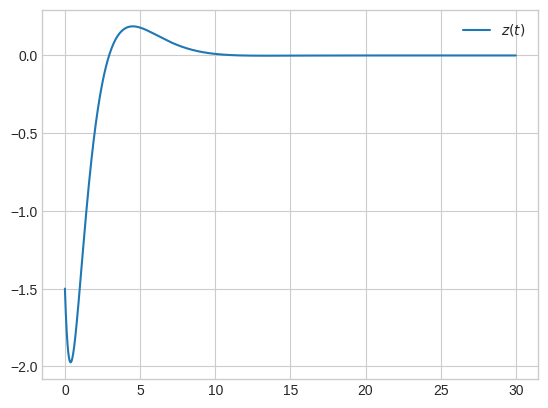
\includegraphics[width=300px]{task_2_outputs.png}
    \caption{\label{fig:task4_3_2}Задание 2. Регулируемый выход.}
\end{figure}
\pagebreak